% 45 minutes, should be ~30 slides or so
\section{Basic Tutorials}

\begin{frame}{Virtual Machine Check}
How are we doing with the Virtual Box images?
\end{frame}

\begin{frame}{Ubuntu Introduction}
\begin{itemize}
  \item User experience oriented version of Linux
  \item Familiar desktop paradigm
  \item TODO: finish after image is ready
\end{itemize}
\end{frame}

\begin{frame}{Ubuntu - Hands On  }
\begin{itemize}
  \item TODO: what do we need to talk about here?
\end{itemize}
\end{frame}

\begin{frame}{Just Enough Python to be Dangerous}
\begin{itemize}
  \item Start a terminal
  \item Run iPython
\end{itemize}
\begin{center}
  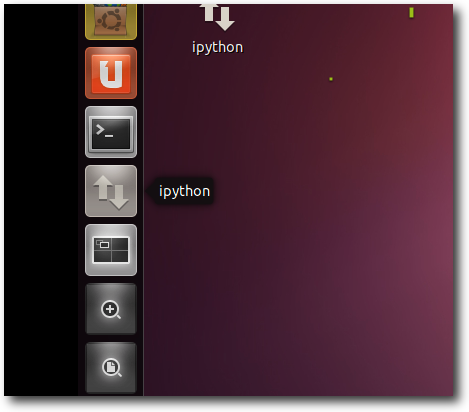
\includegraphics[width=0.5\textwidth]{Images/iPythonLaunch_shadow}
\end{center}
\end{frame}

\begin{frame}{Just Enough Python to be Dangerous}
\begin{center}
  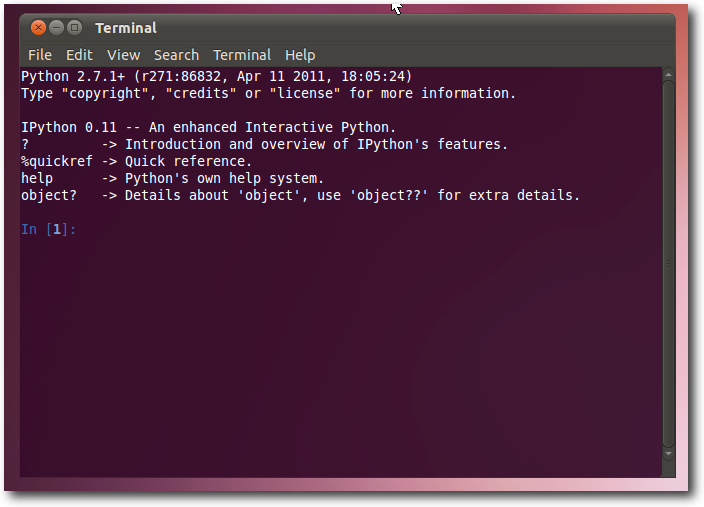
\includegraphics[width=0.5\textwidth]{Images/iPythonWindow_shadow}
\end{center}
\end{frame}

\begin{frame}{Just Enough Python to be Dangerous}
Import the SimpleITK package
\begin{center}
  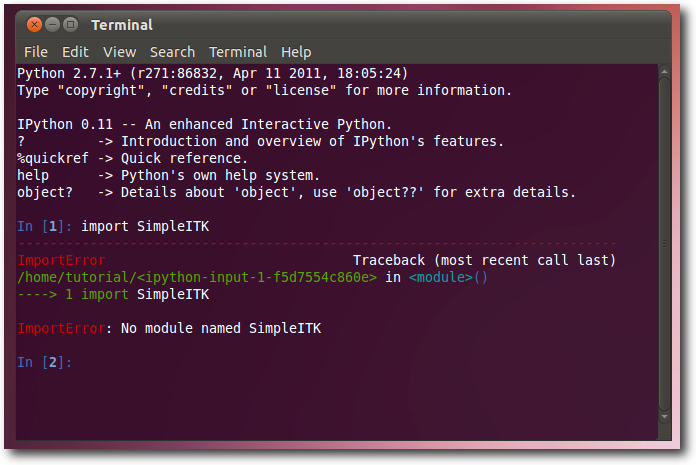
\includegraphics[width=0.5\textwidth]{Images/iPythonImportError_shadow}
\end{center}
What just happened?
\end{frame}

\begin{frame}{Just Enough Python to be Dangerous}
Need to tell iPython where to find SimpleITK\\
See /home/tutorial/.ipython/ipython.py
\begin{center}
  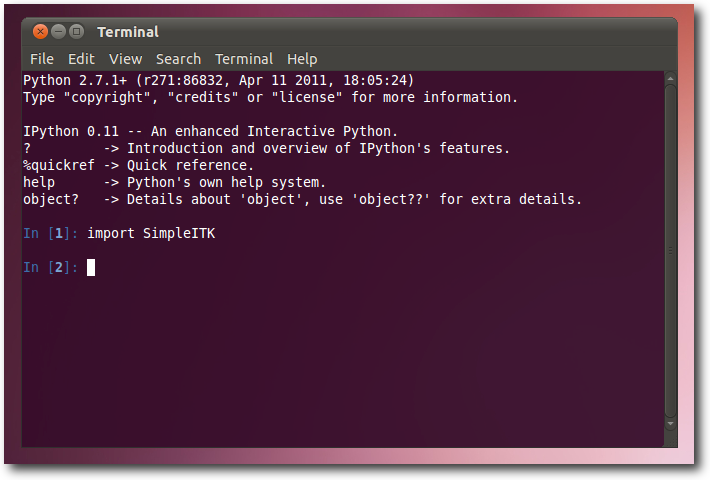
\includegraphics[width=0.5\textwidth]{Images/iPythonWithSimpleITK_shadow}
\end{center}
\end{frame}

\subsection{Image Basics}
\begin{frame}
\frametitle{Image Class}
\end{frame}


\subsection{Input/Output}

\begin{frame}
\frametitle{Read an image}
\end{frame}

\begin{frame}
\frametitle{Write an image}
\end{frame}

\begin{frame}
\frametitle{Display an image}
\end{frame}

\subsection{Filters}

\begin{frame}
\frametitle{Where did the pipeline go?}
\end{frame}

\begin{frame}
\frametitle{How filters work}
\end{frame}




